%%%%%%%%%%%%%%%%%%%%%%%%%%%%%%%%%%%%%%%% 
% SOS Background
%%%%%%%%%%%%%%%%%%%%%%%%%%%%%%%%%%%%%%%% 
\section{Background --- SOS Operating System}
\label{sec:background}
% 
The initial motivation of our work was to provide memory protection
for mote-class sensor nodes running the SOS operating system.
% 
% The design ideas of Harbor are generally applicable however its
% implementation and evaluation are specific to SOS.
% 
We have implemented and evaluated Harbor's protection mechanisms on
SOS, although the ideas should apply elsewhere.
% 
This brief introduction to SOS is useful to fully understand the
implementation of our scheme.
% 
%===================================================
%\subsection{SOS Operating System}
% 
%% Unique resource tradeoffs in the nodes, the distributed and
%% collaborative nature of applications and the remote unattended
%% operation of sensor networks motivate the design of a new class of
%% operating system and run-times.
% 
TinyOS~\cite{levis05t2}, the most popular operating system for sensor
networks, uses reusable software components to implement common
services, but each node runs a statically linked system image.
% 
%% The components are written in the NesC~\cite{gay03nesc} programming
%% language.
% 
%% Mat\'e~\cite{asvm05nsdi}, an application specific virtual machine
%% on top of TinyOS provides limited flexibility to re-task a deployed
%% network using high-level scripts.
% 
SOS has a more traditional architecture: a kernel is
installed on all nodes, and
% 
% The rest of the system and 
application level functionality is implemented by a set of dynamically
loadable binary modules~\cite{ram05sos}.
% 
% In contrast to TinyOS, SOS maintains modularity at the binary level
% without any loss in efficiency.
% 
% This property of SOS makes it particularly attractive to explore
% techniques for isolating software faults.
% 
%% We have implemented the memory protection mechanism on the SOS
%% operating system.
% 
%% The embodiment of the scheme is specific to SOS, however it can
%% easily be applied to the other existing run-times as well
%% (Subsection~\ref{sec:conclude}).
% 
% any operating system that supports dynamically loadable binary
% modules.
% 
% This brief introduction to SOS is useful to fully understand the
% implementation of our scheme.
% 
% 
% 
The kernel is relatively well tested; we assume it is free of
programming errors.
% 
Modules are position independent binaries that implement a specific
task or function, and are less well tested by comparison.
% 
Modules operate on their own state, which is dynamically allocated at
run-time.
% 
An application in SOS is composed of one or more modules interacting
via asynchronous messages or function calls.
% 
Examples of modules are routing protocols, sensor drivers, application
programs, and so forth.
%
%----------------------------------------------------------
\subsection{Module Linking}
\label{sec:soslinking}
%
Any SOS module is linked upon loading with the kernel and other
modules in the system. 
%
%Modules communicate with one another through asynchronous message
%passing or synchronous function calls
%(Figure~\ref{fig:sos_mod_interactions}).
%
The SOS kernel provides a rich set of services such as software
timers, networking, sensor I/O, etc., accessible via a system
call API.
%
The kernel maintains a jump table in program memory that stores the
addresses of system calls (Figure~\ref{fig:sosjmptbl}).
%
The modules are pre-linked to the jump table entries.
%
Thus they do not have to carry any linking information, which reduces
their size.
%
This design also provides flexibility to change the kernel independent
of the modules as long as the consistency of the jump table is maintained.
%

Modules are also linked with one another through function pointer
pointers (Figure~\ref{fig:modinteract}).
%
Every module carries records that indicates the set of functions to
which it wishes to subscribe (from the rest of the system) and the set
of functions that it provides (for the rest of the system).
%
The dynamic linker tracks down and links all the provide-subscribe
function pairs when a module is loaded.
%
\begin{figure}[htpb]
 \centering
  \mbox{
    \subfigure[Jump Table for System
    API]{\label{fig:sosjmptbl}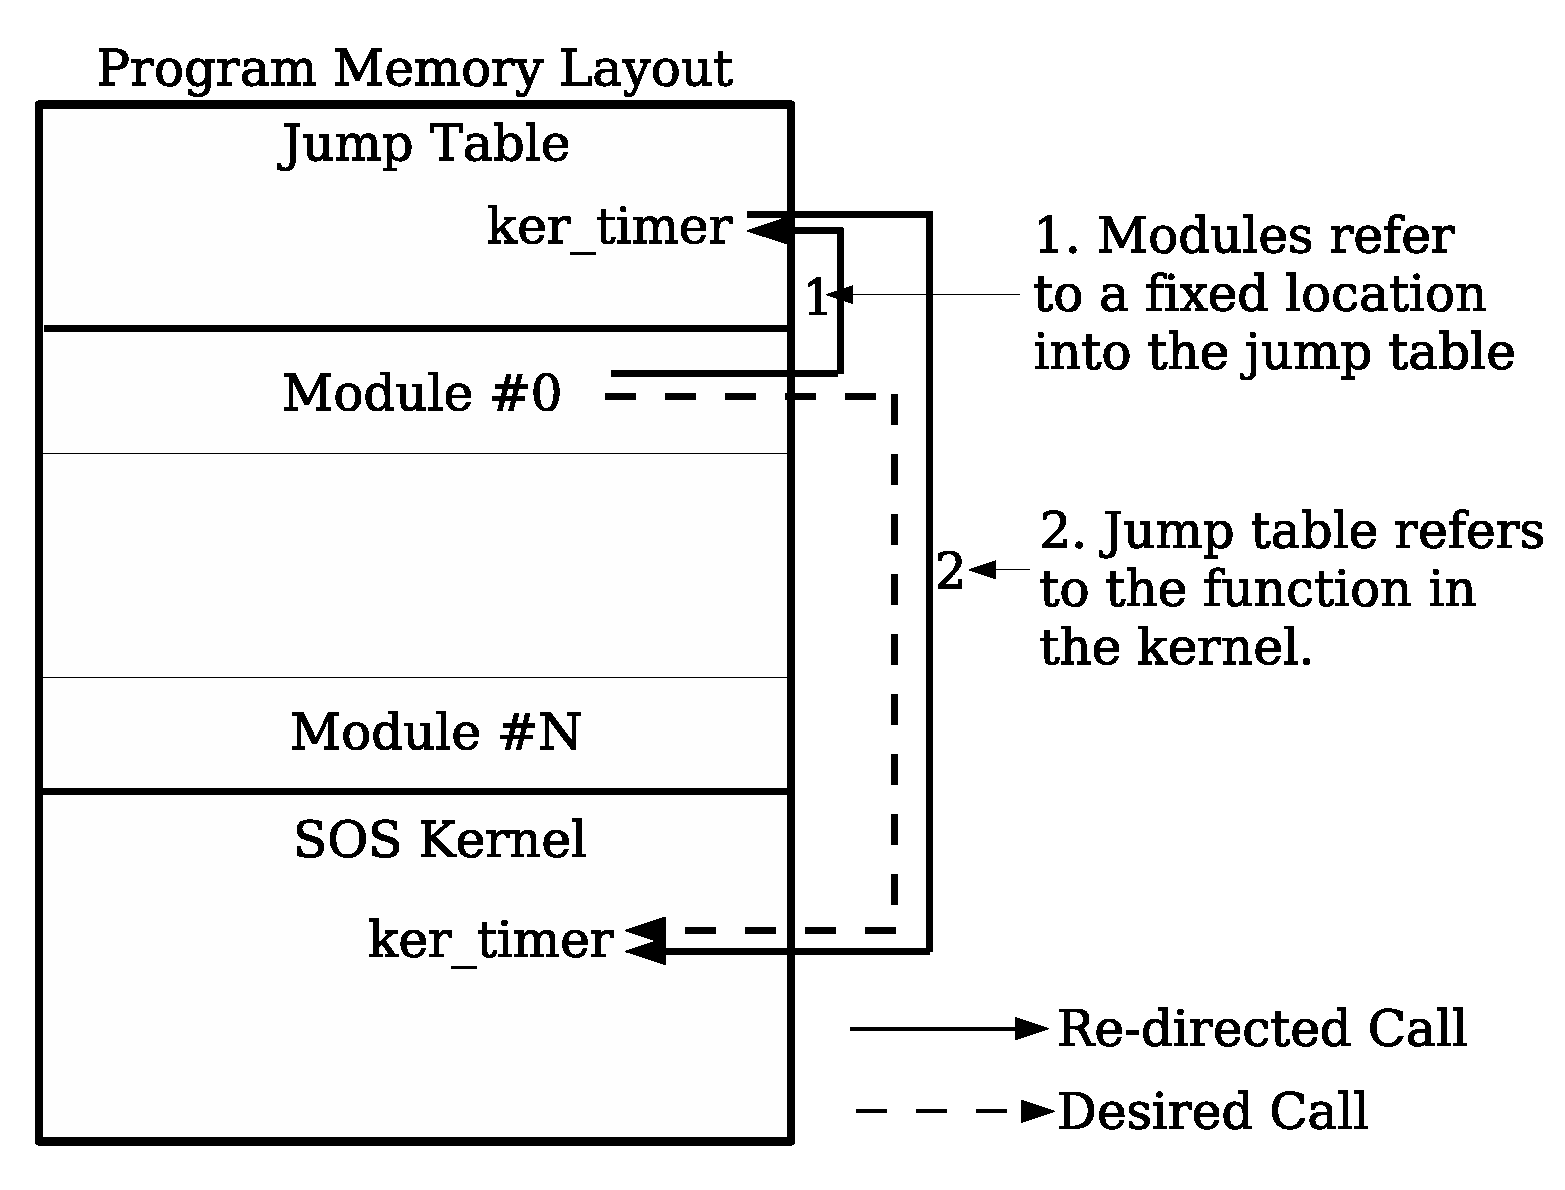
\includegraphics[height=2in,
      keepaspectratio = true]{figures/jumptable.eps}}
    \hspace{0.2in}
    \subfigure[Module
    Interactions]{\label{fig:modinteract}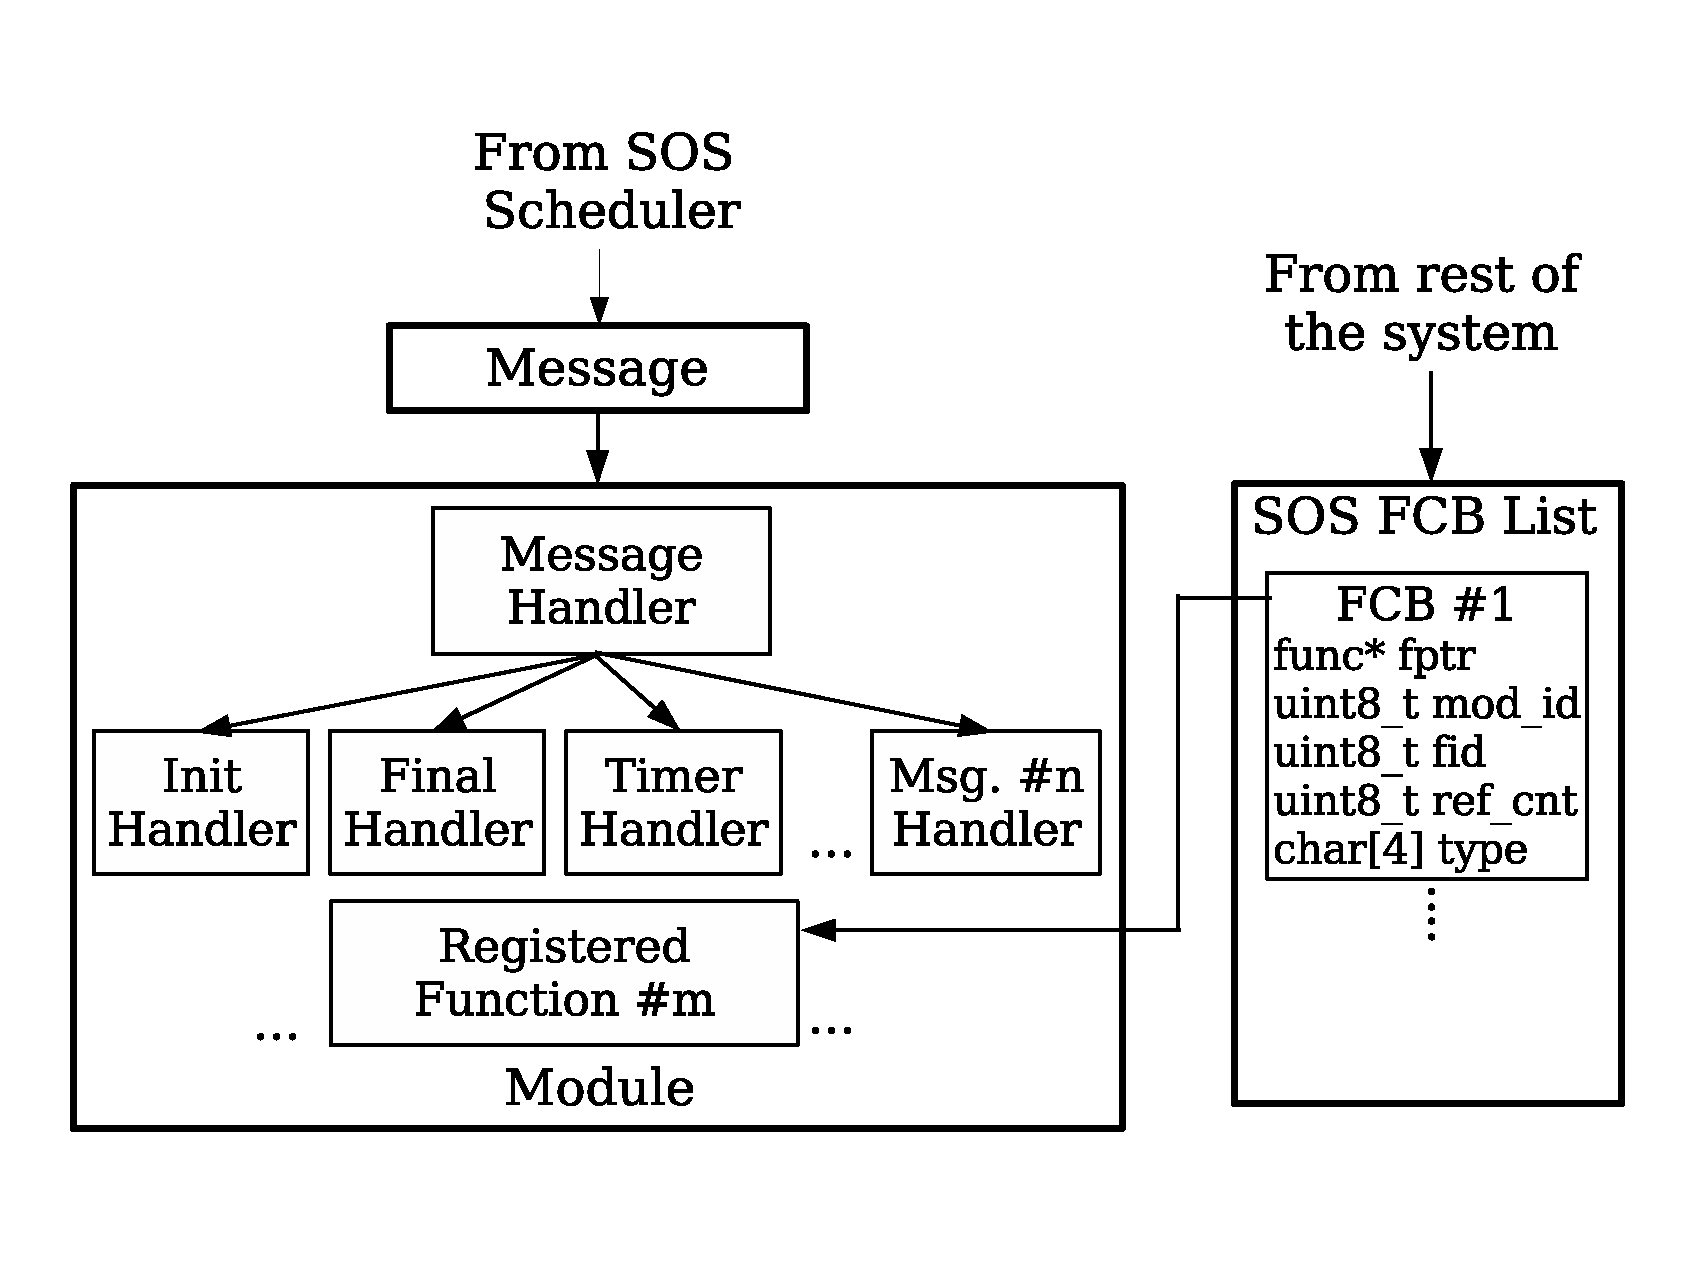
\includegraphics[height=2in,
      keepaspectratio = true]{Figures/module_interactions.eps}}
  }
  \caption{Linking SOS Module}
\end{figure}   
%
% \begin{figure}[htbp]
%   \centering
%   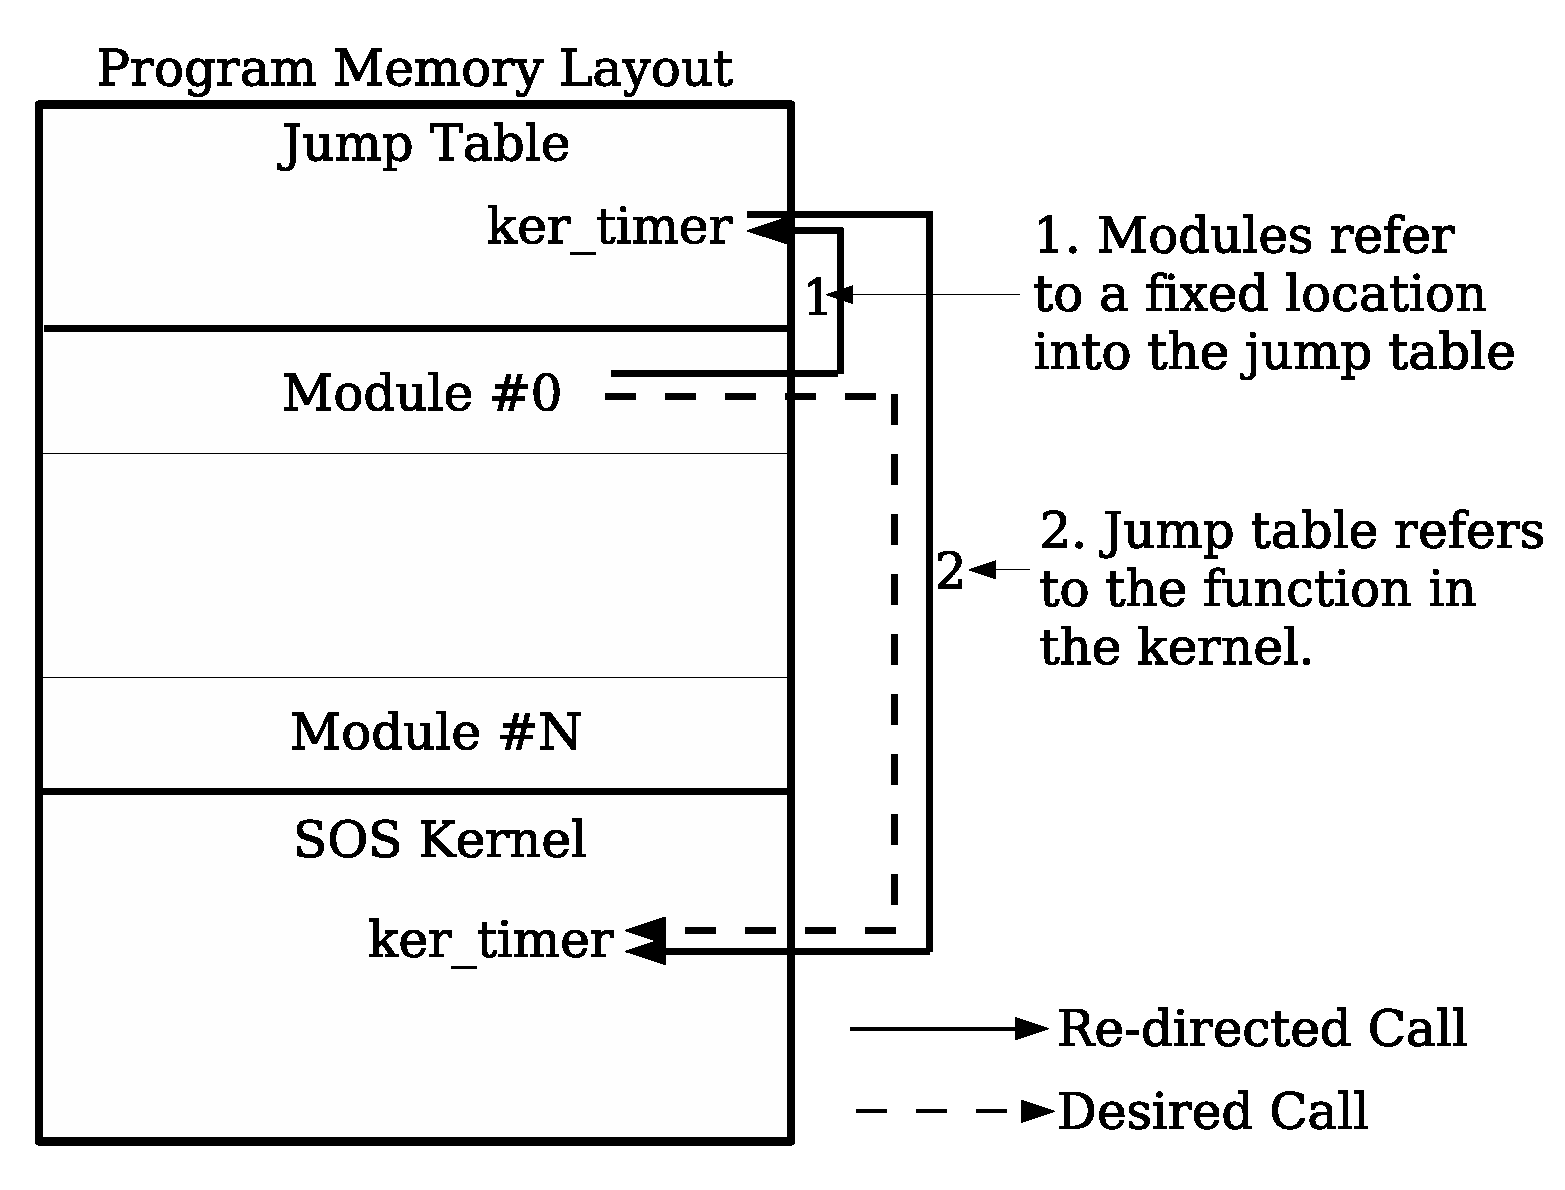
\includegraphics[height = 1.75in,
%   keepaspectratio=true]{figures/jumptable.eps} 
%   \caption{Jump Table for SOS Modules}
%   \label{fig:sosjmptbl}
% \end{figure}
%----------------------------------------------------------
\subsection{Message Passing}
%
The modules in SOS can communicate with other modules and the kernel
through message passing.
%
SOS modules are implemented as message handlers as shown in
Figure~\ref{fig:modinteract}.
%
The messages are annotated with the identity of the destination module
and stored in a FIFO queue within the kernel.
%
The scheduler invokes a handler function in the destination module of
a message.
%
During load time, the modules register the handler function with
the kernel.
%
%All modules are required to implement a message handler.
%
The message handlers execute in the background context.
%
The background context comprises of operations that can only be
interrupted by events occurring in the foreground context (for
e.g. hardware interrupts).
%
%A module can invoke synchronous system calls in the kernel and
%synchronous function calls in the other modules from a message
%handler.
%
After a handler terminates, the execution control is transferred back
to the scheduler.
%
SOS requires cooperative scheduling to share the processor between
multiple executing modules.
%
%---------------------------------------------------------
\subsection{Dynamic Memory Allocation}
% 
The SOS kernel supports dynamic memory allocation.
% 
Dynamic memory is used to store module state and to create messages to
be dispatched to other modules. 
% 
Memory is allocated using a block-based first-fit scheme to minimize
the overhead of the allocation process.
%
The size of the block is platform dependant and is 8 bytes for Mica2
sensor node.
% 
Limited memory forces SOS kernel and user modules to share a common
allocation heap; any static partitioning would be too conservative.
% 
% The dynamic memory is shared by the SOS kernel and the modules.
% 
The kernel therefore tracks ownership of memory blocks.
% 
A block's ownership can also be transferred, allowing
% 
buffers to pass easily through various modules in the system.
% 
% 
%====================================================================== 
% \subsection{System Components}
% % 
% Harbor's four components are shown in Figure~\ref{fig:sys_overview}.
% % 
% %% We first describe overall system operation.
% % 
% The system's input consists of raw user module binaries generated by a
% cross-compiler toolchain.
% % 
% The \emph{binary rewriter} is a desktop application that statically
% analyzes these binaries for potentially unsafe operations and inserts
% run-time checks to sandbox them.
% % 
% The sandboxed binary is then distributed to a network of sensor nodes.
% % 
% A \emph{verifier} running on each node verifies that incoming binaries
% are correctly sandboxed.
% % 
% Verified binaries admitted for execution interact closely
% with Harbor's run-time components, the \emph{memory map manager} and \emph{control flow
%   manager}.
% %
% \begin{figure}[htbp]
%   \centering
%   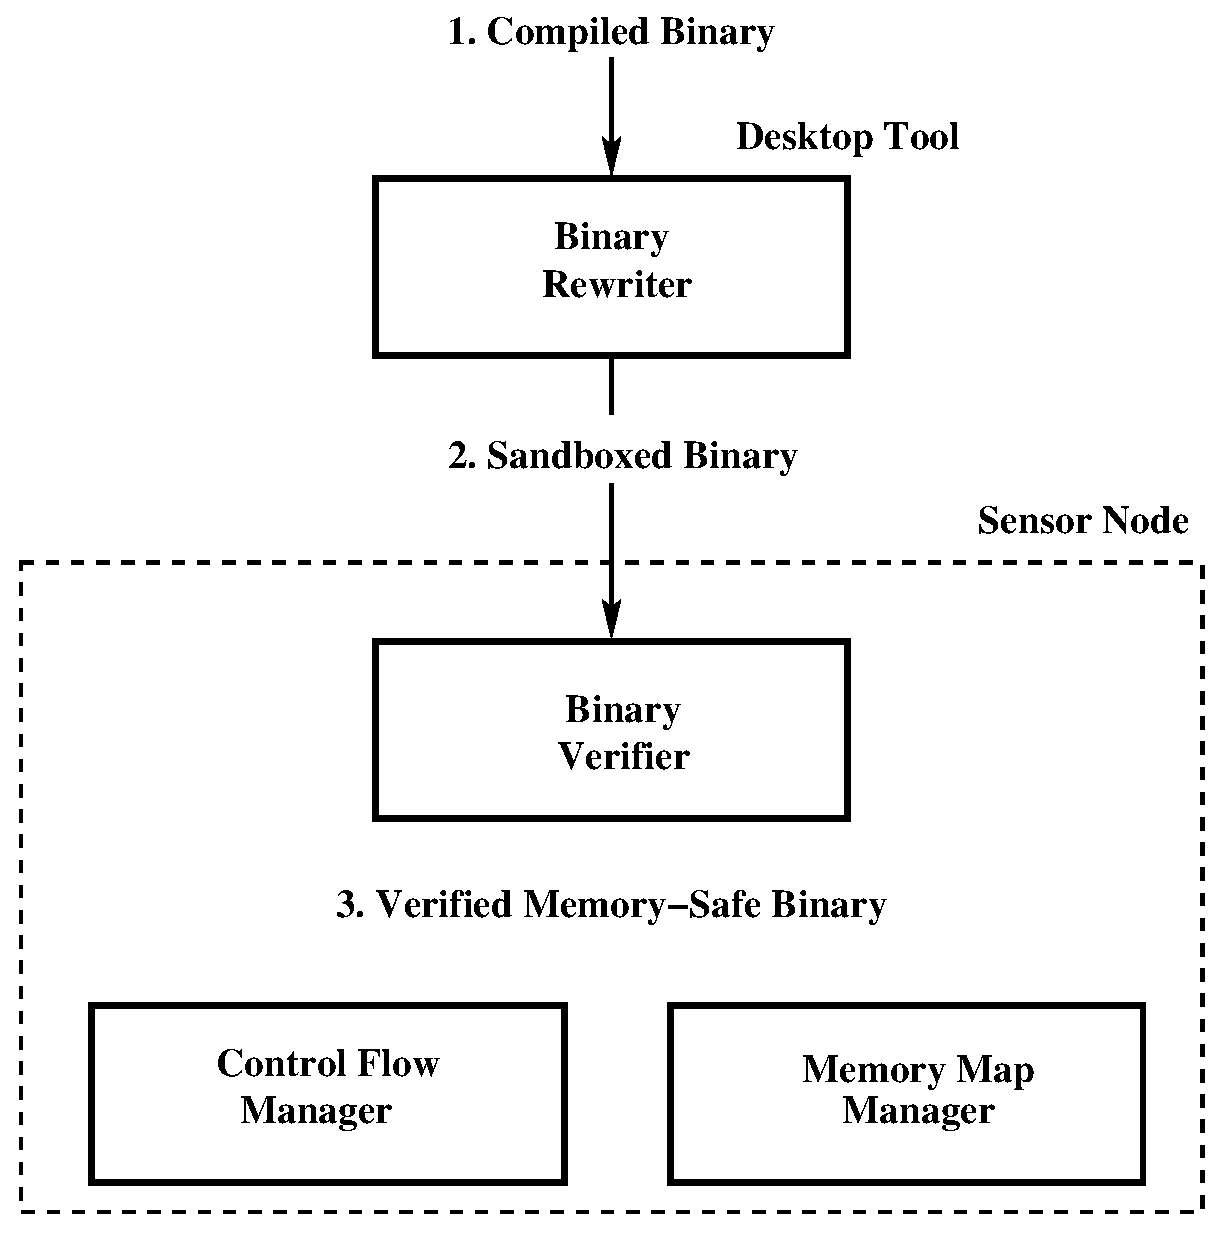
\includegraphics[height = 2.0in, keepaspectratio=true]{figures/sysoverview.eps} 
%   \caption{System Overview}
%   \label{fig:sys_overview}
% \end{figure}
